\chapter{Mapping}\label{chap:mapping}
Mapping is the process of building representations of the environment for
either downstream consumption by autonomy algorithms or for informing humans.
Maps inform decision-making for planning and control algorithms by, for
example, providing information on the surfaces and obstacles, objects with
which the robot can interact, or topological information like how rooms are
connected with one another. If maps of an environment are already provided,
robots can build plans over them without having to build a map themselves;
indeed, they can even localize themselves within these maps simply by
collecting information \emph{in situ} and referencing that information against
prior maps. Mapping also provides humans with an appreciation for what the
robot \emph{sees}, thereby guiding designers or operators of robots with
information about what is possible or information available to the robot.
Therefore, mapinformation for both the purposes of autonomy and design is a
critical linchpin to operating in real environments.

When one considers the quantities of interest to be collected from an
environment, there are two distinct classes: metric (e.g., the physical extents
of an environment) and semantic (e.g., the type of room one is in, or objects
of interest within it). These two categories can inform one another, for
instance a door is typically of a particular height or width, but the inference
required to resolve information in these two classes is remarkably different.
Metric information is frequently resolved using geometric techniques with which
we have become familiar in Chapter \ref{chap:sensors}, whereas semantic
information is typically obtained through machine learning techniques. For the
purposes of this text, we will focus almost exclusively on the problem of
metric mapping due to the prevailing importance of this information as it
relates to robotic planners and localization, but semantic mapping is a rich
field with an increasing importance to developing robotic autonomy; 
greater distinctions between these types of maps will be discussed in
Section \ref{sec:maps}.

With respect to metric mapping, range sensors have emerged as one of the most
effective sensors to make robots autonomous. Range data can be collected into
``scans'' from a sensor, each of which consists of a list of points that we
term a point cloud. Point clouds makes the construction of a 3D model of the
robot's environment straightforward; measurements on the environment are
inherently metric and require no ``front-end'' processing, as images from a
camera might require to extract such information. Furthermore, sensors that
output point cloud data are both quite accurate and increasingly common on
robotic platforms: the Velodyne 3D automotive lidar sensor that combines 64
scanning lasers into one package was key in mastering the DARPA Grand
Challenge, and no team operated without lidars as part of their solution in the
recent DARPA Subterranean Challenge. So for both wide-area and close-corridor
operation, 3D lidar has become a standard. There is one hitch with lidars: most
of them are built out of rotating laser arrays, which means that a moving
sensor will collect information from the environment at different rotation
angles, thereby \emph{aliasing} the lidar measurements with the motion of the
sensor. This motion aliasing can be removed from the lidar data, but is
negligible if the motion of the sensor is slow enough. However, there are
sensors that provide range data without this limitation, such as RGB-D (color
plus depth) cameras.  Furthermore, 3D range data has become even more important
in robotics with the advent of cheap (priced at a tenth of the price of the
cheapest 2D laser scanner) RGB-D cameras. In this chapter we will largely
ignore the source of range data, and will instead focus on algorithms that
operate over these data.

The mapping problem itself also ranges from trivial (when localization is
perfect) to arbitrarily complex, performing the equivalent of cartography in
which the tasks of localizing oneself and mapping the environment are closely
intertwined. While the problem of ``simultaneous localization and mapping''
will be introduced in Chapter \ref{chap:slam}, Section \ref{sec:ICP} describes
one of the key algorithms that is used to infer relative pose between
consecutive measurements by a process known as scan matching. 

Point cloud data allows fitting of lines and planes using RANSAC, which can
serve as features in EKF-based localization, but can also be used for improving
odometry, loop-closure detection, and mapping. Point cloud data can also be
probabilistically fused into voxel occupancy grids and dense surface
representations, which inform planning and design. The goals of this chapter
are:

\begin{itemize}
    \item introduce the Iterative Closest Point (ICP) algorithm for matching point clouds as an example of sparse mapping;
    \item show how ICP can be improved by providing initial guesses via RANSAC;
    \item use point clouds to generate dense maps built through occupancy grids; and
    \item demonstrate RGB-D mapping, another dense mapping technique that results in surface representations.
\end{itemize}

\section{Map representations}\label{sec:maps}
In order to plan a path, we need to represent the environment digitally. We
differentiate between two complementary approaches: discrete and continuous
approximations. In a discrete approximation, a map is sub-divided into sections
of equal (e.g., a grid or hexagonal map) or differing sizes (e.g., rooms in a
building). The latter maps are also known as \textsl{topological maps} or
\textsl{graph-based maps}.\index{Topological map}\index{Graph-based map}
Discrete maps lend themselves well to a graph representation. Here, every
region of the map corresponds to a vertex (also known as a ``node''), which are
connected by edges if a robot can navigate from one vertex to the other. For
example a road-map is a topological map with intersections as vertices and
roads as edges, labeled with their length (\cref{fig:pathproblem}).
Computationally, a graph might be stored as an adjacency or incidence
list/matrix. A continuous approximation requires the definition of inner
(obstacles) and outer boundaries, typically in the form of a polygon, whereas
paths can be encoded as sequences of points defined by real numbers. Despite
the memory advantages of a continuous representation, discrete maps are the
dominant representation in robotics.

There is no one correct choice for choosing a map representation, and each
application might require a different solution that could utilize a combination
of different map types.

Discrete and continuous representations are often matched together in clever ways. For example, roadmaps for GPS systems are stored as topological maps that store the GPS coordinates of every vertex, but might also contain overlays of aerial and street photography. These different maps are then used at different stages of the path planning stage.


\section{Iterative Closest Point for Sparse Mapping}
In its simplest form, a map can be created from slices of 2D range data such as obtained from a laser scanner. In the absence of a precise estimate of motion between two measurements, for example provided by odometry or IMU measurements, the challenge is to associate subsequent scans. 

A standard solution to this problem is known as the \emph{Iterative Closest Point} (ICP)\index{Iterative Closest Point}\index{ICP} algorithm. It was presented in the early 1990s for registration of 3D range data to CAD models of objects. A more in-depth overview of what is described here is given in \cite{rusinkiewicz01}. The key problem can be reduced to finding the best transformation that minimizes the distance between two sets of measurements.

In robotics, ICP found an application to match scans from 2D laser range
scanners. For example, the transformation that minimizes the error between two
consecutive snapshots of the environment is proportional to the motion of the
robot. This is a hard problem as it is unclear, which points in the two
consecutive snapshots are ``pairs", which of the points are outliers (due to
noisy sensors), and which points need to be discarded as not all points overlap
in both snapshots. Stitching a series of snapshots together theoretically
allows to create a 2D map of the environment. This is difficult, however, as
the error between every snapshots --- similar to odometry --- accumulates.
The ICP algorithm also works in 3D where it allows to infer the change in 6D
pose of a camera and creation of 3D maps. In addition, ICP has proven useful
for identifying objects from a database of 3D objects. Furthermore, the ICP
algorithm can be used to stitch consecutive range images together to create a
3D map of the environment \cite{henry2010rgb}. 

Before providing a solution to the mapping problem, we will focus on the ICP algorithm to match two consecutive frames. Variants of the ICP algorithm can be broken down into six consecutive steps:
\begin{enumerate}
    \item Selection of points in one or both meshes or point clouds.
    \item Matching/Pairing these points to samples in the other point cloud/mesh.
    \item Weighting the corresponding pairs.
    \item Rejecting certain pairs.
    \item Assigning an error metric based on the point pairs.
    \item Minimizing the error metric.
%    \item Point Selection.
\end{enumerate}
Depending on the number of points generated by the range sensor, it might make sense to use only a few selected points to calculate the optimal transformation between two point clouds, and then test this transformation on all points. Depending on the source of the data, it also turns out that some points are more suitable than others as it is easier to identify matches for them. This is the case for RGB-D data, where SIFT features have been used successfully. This is also the case for planar objects with grooves, where sampling should ensure that angles of normal vectors of sampling points are broadly distributed. Which method to use is therefore strongly dependent on the kind of data being used and should be considered for each specific problem.

\paragraph{Matching Points}
The key step in ICP is to match a point to its corresponding point in a different measurement. For example, a laser scanner hits a certain point at a wall with its 67th ray. After the scanner has been moved by 10 cm, the closest hit on the wall to this point might have been by the 3rd ray of the laser. Here, it is actually very unlikely that the laser hits the exact same point on the wall twice, therefore introducing a non-zero error even for an optimal pairing. Prominent methods involve finding the closest point in the other point cloud or finding the intersection of the source points' normal with the destination surface (for matching point clouds to meshes). More recently, SIFT has allowed to match points based on their visual appearance. Similarly to sorting through SIFT features, finding the closest matching point can be accelerated by representing the point cloud in a k-d tree.

\paragraph{Weighting of Pairs}
As some pairs are better matches than others, weighting them in some principled way can drastically improve the quality of the resulting transformation. One approach is to give more weight to points that have smaller distances from each other. Another approach is to take into account the color of the point (in RGB-D images) or use the distance of their SIFT features (weighting pairs with low distances higher than pairs with high distances). Finally, expected noise can be used to weight pairings. For example, the estimates made by a laser scanner are much more faithful when taken orthogonally to a plane than when taken at a steep angle.

\paragraph{Rejecting of Pairs}
A key problem in ICP are outliers either from sensor noise or simply from incomplete overlap between two consecutive measurement frames. A common approach to deal with this problem is to reject pairings when one of the points lies on a boundary of the point cloud, as these points are likely to match with points in non-overlapping regions. As a function of the underlying data, it might also make sense to reject pairings with too high of a distance. This is a threshold-based equivalent to distance-based weighting as described above.

\paragraph{Error Metric and Minimization Algorithm}
After points have been selected and matched, and pairs have been weighted and rejected, the match between two point clouds needs to be expressed by a suitable error metric which will then need to be minimized. One straightforward approach for this is to consider the sum of squared distances between each pair. This formulation can often be solved analytically. Let
\begin{eqnarray}
A=\{a_1,\ldots,a_n\}\\
B=\{b_1,\dots,b_n\}
\end{eqnarray}
be point clouds in $ \mathbb{R}^n$. The goal is now to find a vector $ t \in \mathbb{R}^n$ so that an error function $ \phi(A+t,B)$ is minimized. In 6D (translation and rotation), an equivalent notation can be found for a transformation (see forward kinematics). An error function for the squared distance is then given by
\begin{equation}
\phi(A+t,B)=\frac{1}{n}\sum_{a \in A}\|a+t-N_B(a+t)\|^2
\end{equation}
Here $ N_B(a+t)$ is a function that provides the nearest neighbor of $ a$ translated by $ b$ in $ B$.  A key problem now is that the actual value of $t$ affects the outcome of the pairing. What might look like a good match initially often turns out not be the final pairing. A simple numerical approach to this problem is to find $ t$ iteratively.

Initially $t=0$ and nearest neighbors/pairings are established. We can now calculate a $ \delta t$ that optimizes the least-square problem based on this matching using any solver available for the optimization problem (for a least-square solution $ \delta t$ can be obtained analytically by solving for the minimum of the polynomial by setting its derivative to zero). We can then shift all points in $ A$ by $ \delta t$ and start over. That is, we calculate new pairings and derive a new $ \delta t$.  We can continue to do this, until the cost function reaches a local minimum.

Instead of formulating the cost function as a ``point-to-point'' distance, a ``point-to-plane'' has become popular. Here, the cost function consists of the sum of squared distances from each source point to the plane that contains the destination point and is oriented perpendicular to the destination normal. This particularly makes sense when matching a point cloud to a mesh/CAD model of an object. In this case there are no analytical solutions to finding the optimal transformation, but any optimization method (such as Levenberg-Marquardt) can be used.

\section{Octomap: dense mapping of voxels}
For mapping obstacles, the most common map is the \textsl{occupancy grid
map}\index{Occupancy grid map}. In a grid map, the environment is discretized
into \emph{voxels} of arbitrary resolution, e.g. 1cm x 1cm, upon which obstacles are
marked. In a probabilistic occupancy grid, grid cells can also be marked with
the probability that they contain an obstacle. This is particularly important
when the position of the robot that senses an obstacle is uncertain.
Disadvantages of grid maps are their large memory requirements as well as the
computational time required to traverse data structures with large numbers of
vertices. A solution to this is storing the grid map as a \textsl{k-d
tree}.\index{k-d tree (data structure)} A k-d tree recursively breaks the
environment into $k$ pieces, subject to a subdivision rule (e.g., only
subdivide a space if it is between 5-95\% occupied). For $k=4$, an area that
fits the subdividing criteria would be subdivided into four pieces. Each of
these pieces can again be subdivided into four pieces and so on, until the
maximum allowable resolution is reached or the subdivision criteria no longer
applies. These pieces can be stored in a graph with each vertex having four
children, corresponding to the four pieces the space represented by the vertex
is broken into, unless it is a leaf of the tree. This data structure is
attractive because not all vertices need to be broken down to the smallest
possible resolution. Instead, only areas which contain obstacles need to be
subdivided. A grid map containing obstacles and the corresponding k-d tree are
shown in \cref{fig:gridvskdtree}. To capture 3D data, this representation can
be extended to a 8-d tree, also known as \textsl{Octree}\index{Octree}. 


\begin{figure}
    \centering
    % \includegraphics[width=\textwidth]{figs/gridvskdtree.png}
    \def\svgwidth{\textwidth}
    \import{./figs/}{gridvskdtree.pdf_tex}
    \caption{A grid map and its corresponding quadtree (k-d tree).\label{fig:gridvskdtree}}
\end{figure}

The values of each entry in the k-d tree is the probability that the particularly
specified voxel is occupied. Note that this probability may be calculated
through any number of sensor models, such as absolute thresholding or using a
probabilistic field-of-view sensor model. Absolute thresholding determines
that a voxel is occupied if the absolute count of points measured
by the sensor within a voxel is greater than a threshold. An improvement on this is
to use a probabilistic model wherein a false positives
incidence rate and false negative incidence rate are used to calculate the probability
that a sensor's measurements indicate that a particular voxel is filled. Either way,
these techniques result in a map that is probabilistically fused over a sequence of
measurements to indicate filled and unfilled space in the form of a volumetric map.


\section{RGB-D mapping: dense mapping of surfaces}
While occupancy grid mapping using a technique such as Octomap is efficient for
planning, there are some drawbacks of this technique. First, it can be
immediately observed that the map voxels are of a fixed resolution and
fundamentally cannot resolve small obstacles at any smaller scale than that of
the voxels; that is, small obstacles will appear larger. Furthermore,
high-frequency information within the voxel that may be relevant to planning,
such as surface curvatures, are unresolvable.  However, this information seems
out of reach for any voxelized representation of the environment. The
resolution to this paradox is to populate the value of voxels not with
probability of a voxel's being occupied, but rather the \emph{most probable
distance} to the nearest surface. If for a particular range scan, a surface
lies beyond a certain voxel, that distance is positive, and if a surface lies
in front of a certain voxel, that distance is negative. See Figure
\ref{fig:sdf} for an example of this mathematical construction, which is known
as a \emph{signed distance field} (SDF). The SDF is generated by following the
distance along a ray to the surface and entering that value into the voxel, and
incrementally probabilistically updating the values in the voxel as frames are
consumed from the depth channel.  Note that the SDF provides an implicit
representation of a surface as can be seen in Figure \ref{fig:sdf}. In this
figure the notion of ``truncation'' is also motivated, wherein voxels that
would have a value above a certain threshold known as a truncation distance are
left unfilled; this is a frugal use of memory and results in a speedup for
reconstruction algorithms. It also is required to avoid surfaces interfering
with one another.  An SDF which is pruned in this way is known as a ``truncated
SDF'' (TSDF).

\begin{figure}
    \centering
    \def\svgwidth{0.8\textwidth}
    \import{./figs/}{sdf.pdf_tex}
    \caption{Schematic of the generation of a TSDF based on 2D range data from a sensor. Voxels are only populated with distances that lie within the ``truncation distance.''\label{fig:sdf}}
\end{figure}

The TSDF can naturally represent multiscale obstacles, and provides an added
benefit for planning algorithms: it provides the distance to the nearest
obstacle at the same time! This is helpful as distance to obstacles can be used
as a risk metric in planning algorithms (i.e.\ it is often advantageous to
maintain maximal distance from obstacles over a trajectory, which can be easily
obtained from the TSDF). There are two significant downsides of this technique,
however.  First, it requires highly accurate pose information, frequently
meaning ICP must be performed for each scan from the sensor. Second is that
implicit representation of surfaces do not admit straightforward visualizations
of the 3D maps. In order to accomplish this, a rendered is required to operate
on the TSDFs, which result in maps such as \cref{fig:kintinuous}, which is using
the method of \cite{whelan2013robust}.  The resulting visualizations can be
surprisingly high-resolution even over coarse voxelization of the environment.
Together with RGB information, it is possible to create complete 3D walk
throughs of an environment.

\begin{figure}
    \centering
    \includegraphics[width=\textwidth]{figs/kintinous}
    \caption{Fused point cloud data from a walk trough of an office environment using ``Kintinious''. Picture courtesy of John Leonard.\label{fig:kintinous}}
\end{figure}


The problem with using ICP continuously to generate these maps is that errors
in each transformation propagate into the maps generation process in the form
of map drift. Here, the SLAM algorithm (Chapter
\ref{chap:slam}) can be used to correct previous errors
once a loop closure is detected, but the update of TSDFs on the trigger of a loop
closure requires both the continuous retaining and global reprocessing of all
data used to generate the TSDFs that would be effected by the loop closure, which
is a high price to pay.

%This form of RGB-D mapping uses a variant of ICP that is enhanced by SIFT features for point selection and matching. Maps are build incrementally. SIFT features, and their spatial relationship, are used for detecting loop closures. %Once a loop closure is detected, an additional constraint is added to the pose graph and a SLAM-like optimization algorithm corrects the pose of all previous observations.

As ICP only works when both point clouds are already closely aligned, which might not be the case for a fast moving robot with a relatively noisy sensor (the XBox Kinect has an error of 3cm for a few meters of range vs. millimeters in laser range scanners), RGB-D Mapping uses RANSAC to find an initial transformation. Here, RANSAC works as for line fitting: it keeps guessing possible transformations for 3 pairs of SIFT feature points and then counts the number of inliers when matching the two point clouds, one of which being transformed using the random guess.


\section*{Take-home lessons}
\begin{enumerate}
\item The challenge in mapping an environment originates from the uncertainty in both localization and sensing.
\item Techniques that are used to overcome uncertainty in localization and sensing can in turn be used to increase confidence in the former. For example, given robust features such as corners or walls, ICP results can be used to improve odometry estimates.
\item In the absence of reliable localization, the mapping problem turns into the simultaneous localization and mapping problem that is addressed in Chapter \ref{chap:slam}.
\end{enumerate}

\section*{Exercises}
\begin{enumerate}
\item Simulate a Lidar sensor in a simulator of your choice.Devise a grid-map structure that will allow you to draw the robot's position. Use the constant angular offset of your Lidar sensor and the pose of the robot to compute map coordinates for each reading.
\item Run a simulated robot in an obstacle course and record a map using your simulated Lidar. Implement the ICP algorithm described above to estimate the translation between consecutive scans and compare them with your odometry estimate. 
\item Use ICP to improve the robot's state estimate for different settings of wheel-slip in your simulation.  
\end{enumerate}
